\section{Implementation Approach}
Clouds are comprehensible indicators for telling the weather. 
They offer many visible features to make an rough prediction of the weather conditions, or weather changes to come.
As described in \sectionref{section:clouds:types}, some cloud types only form under specific conditions.
Also, whenever certain clouds are present, \gls{precipitation} is shortly followed, as it is with altostratus clouds.
\\
Those factors allow a prediction of the weather, but for this project, the process is reversed.
The given data is not an image of clouds, but meteorological measurement data, and the desired outcome is not a prediction, but an image of clouds.

\begin{figure}[H]
    \centering
    \begin{minipage}{0.47\linewidth}
        \begin{tikzpicture}
            \tikzset{edge/.style = {-{Latex[length=3mm]},shorten >= -4pt}}
            \tikzset{shortedge/.style = {shorten <=-4pt,shorten >= -4pt}}
            \tikzset{shortshortedge/.style = {shorten <=-5.5pt,shorten >= -5.3pt}}
            \tikzset{shortshortedge2/.style = {shorten <=-4.5pt,shorten >= -4.5pt}}

            % rainy clouds
            \node (cloud1) at (0.5, 2.0) {};
            \node (cloud2) at (0.8, 2.2) {};
            \node (cloud5) at (1.6, 2.0) {};
            \node (cloud3) at (1.0, 1.9) {};
            \node (cloud4) at (1.3, 2.2) {};
            \node[cloud,fill=gray!30,cloud puffs=9, cloud, minimum width=0.5cm, minimum height=0.2cm, align=center, draw] (cloud) at (cloud1) {};
            \node[cloud,fill=gray!30,cloud puffs=9, cloud, minimum width=0.5cm, minimum height=0.2cm, align=center, draw] (cloud) at (cloud2) {};
            \node[cloud,fill=gray!30,cloud puffs=9, cloud, minimum width=0.5cm, minimum height=0.2cm, align=center, draw] (cloud) at (cloud5) {};
            \node[cloud,fill=gray!30,cloud puffs=12, cloud, minimum width=1.0cm, minimum height=0.7cm, align=center, draw] (cloud) at (cloud3) {};
            \node[cloud,fill=gray!30,cloud puffs=12, cloud, minimum width=0.8cm, minimum height=0.5cm, align=center, draw] (cloud) at (cloud4) {};
            \draw[edge] (2.5, 2) -- (3.5,2);
            \node at (5,2) {rain ahead};

            % clear clouds
            \node (cloud1) at (0.5, 0.0) {};
            \node (cloud2) at (0.9, 0.2) {};
            \node (cloud5) at (1.6, 0.0) {};
            \node[cloud,fill=white,cloud puffs=9, cloud, minimum width=0.5cm, minimum height=0.2cm, align=center, draw] (cloud) at (cloud1) {};
            \node[cloud,fill=white,cloud puffs=9, cloud, minimum width=0.5cm, minimum height=0.2cm, align=center, draw] (cloud) at (cloud2) {};
            \node[cloud,fill=white,cloud puffs=9, cloud, minimum width=0.5cm, minimum height=0.2cm, align=center, draw] (cloud) at (cloud5) {};
            \draw[edge] (2.5, 0) -- (3.5,0);
            \node at (5.7,0) {fair weather ahead};

        \end{tikzpicture}
        \captionof{figure}{Weather information based on visual data.}
        \label{img:tikz:impl:data1}
    \end{minipage}        
    \hfill
    \begin{minipage}{0.47\linewidth}
        \begin{tikzpicture}
            \tikzset{edge/.style = {-{Latex[length=3mm]},shorten >= -4pt}}
            \tikzset{shortedge/.style = {shorten <=-4pt,shorten >= -4pt}}
            \tikzset{shortshortedge/.style = {shorten <=-5.5pt,shorten >= -5.3pt}}
            \tikzset{shortshortedge2/.style = {shorten <=-4.5pt,shorten >= -4.5pt}}

            % rainy clouds
            \node (cloud1) at (4.5, 2.0) {};
            \node (cloud2) at (4.8, 2.2) {};
            \node (cloud5) at (5.6, 2.0) {};
            \node (cloud3) at (5.0, 1.9) {};
            \node (cloud4) at (5.3, 2.2) {};
            \node[cloud,fill=gray!30,cloud puffs=9, cloud, minimum width=0.5cm, minimum height=0.2cm, align=center, draw] (cloud) at (cloud1) {};
            \node[cloud,fill=gray!30,cloud puffs=9, cloud, minimum width=0.5cm, minimum height=0.2cm, align=center, draw] (cloud) at (cloud2) {};
            \node[cloud,fill=gray!30,cloud puffs=9, cloud, minimum width=0.5cm, minimum height=0.2cm, align=center, draw] (cloud) at (cloud5) {};
            \node[cloud,fill=gray!30,cloud puffs=12, cloud, minimum width=1.0cm, minimum height=0.7cm, align=center, draw] (cloud) at (cloud3) {};
            \node[cloud,fill=gray!30,cloud puffs=12, cloud, minimum width=0.8cm, minimum height=0.5cm, align=center, draw] (cloud) at (cloud4) {};
            \draw[edge] (2, 2) -- (3.5,2);
            \node at (0,2) {rain ahead};

            % clear clouds
            \node (cloud1) at (4.5, 0.0) {};
            \node (cloud2) at (4.9, 0.2) {};
            \node (cloud5) at (5.6, 0.0) {};
            \node[cloud,fill=white,cloud puffs=9, cloud, minimum width=0.5cm, minimum height=0.2cm, align=center, draw] (cloud) at (cloud1) {};
            \node[cloud,fill=white,cloud puffs=9, cloud, minimum width=0.5cm, minimum height=0.2cm, align=center, draw] (cloud) at (cloud2) {};
            \node[cloud,fill=white,cloud puffs=9, cloud, minimum width=0.5cm, minimum height=0.2cm, align=center, draw] (cloud) at (cloud5) {};
            \draw[edge] (2.5, 0) -- (3.5,0);
            \node at (0.7,0) {fair weather ahead};
            
        \end{tikzpicture}
        \captionof{figure}{Visual construction based on weather information.}
        \label{img:tikz:impl:data2}       
    \end{minipage}
\end{figure}

\noindent
For any given day to render, an implementation would require data from that day but also from the near future of that day.
So, in order to render a cloud image for day $x$, a potential algorithm could look like this.
Note that the listing below describes only an idea and is by no means final or compulsory.

\begin{lstlisting}[language=HLSL, caption=Pseudo-code of cloud render algorithm., label=lst:pseudo:algorithm]
// weather data including 7-day forecast
WeatherData data;

function renderClouds(Day x) {
    if (x > TODAY + 7) throw;

    d1 = data.getDataFor(x);
    d2 = data.getDataFor(x + 1);
    d3 = data.getDataFor(x + 2);
    // and so on...

    // sophisticated checks about current and future conditions:
    if (d1.fairWeather && d2.fairWeather)
        return renderer.clearSky();
    if (d1.fairWeather && d2.isRaining)
        return renderer.cloudsOnclearDayBeforeRain();
    if (d1.isRaining)
        return renderer.cloudsOnRainyDay();
    if (d2.isRaining) 
        return renderer.cloudsBeforeRainyDay();
    if (d3.isRaining) 
        return renderer.clouds2DaysBeforeRainyDay();
    // and so on...
    
}
\end{lstlisting}

\clearpage

\subsection{Look-Ahead Issue}
The approach as described above relies on having data from a couple of days ahead of time. Assumed that number of days is $t$, then the weather data for day $x$ could only be rendered $t$ days after $x$.
That would mean, for such an approach to work, the weather of today can not be rendered before $t$ days later.
\\
In this case however, the weather measurement data retrieved from \emph{meteoblue} also contains a seven-day weather forecast. 
Given that $t$ is less than or equal to seven and an implementation still produces accurate cloud imagery, it would no longer be an issue.

\subsection{Layers of Cloud Shaders}
As identified in \sectionref{section:clouds:types}, most of the clouds in the troposhpere only appear at certain \gls{altitude}s.
The high-level clouds are all of type \emph{cirrus}.
The mid-level clouds are both of type \emph{alto} and similar in look, while most of the low-level clouds belong to the \emph{cumulus} family.
\\
This leads to the conclusion that some of the cloud types could be combined into a single layer and rendered by the same shader.
Exception to that are only the two larger types that span over multiple height levels: nimbostratus and cumulonimbus. For those, a more unique solution has to be found.

\begin{figure}[H]
    \centering
    \begin{tikzpicture}[scale=1]
        \tikzset{edge/.style = {-{Latex[length=3mm]},shorten >= -4pt}}
        \tikzset{shortedge/.style = {shorten <=-4pt,shorten >= -4pt}}
        \tikzset{icon/.style = {font=\Large}}

        % icons
        \node[red,icon] (cam) at (0.1, 5.2) {\faVideoCamera};
        \node[red,yshift=-0.5cm,xshift=-0.3cm] at (cam) {camera};
        \draw (0.5,5.45) -- (2,7);
        \draw (0.5,4.95) -- (2,3.5);

        % cloud layer boxes
        \draw (3,7) rectangle (10,6.2);
        \draw (3,6) rectangle (10,5.2);
        \draw (3,5) rectangle (10,4.2);
        \draw (3,4) rectangle (10,2.2);
        \node at (6.5,6.6) {cirrus layer};
        \node at (6.5,5.6) {alto layer};
        \node at (6.5,4.6) {stratus layer};
        \node at (6.5,3.1) {fog layer};

        % houses
        \node[black!40] at (4.9, 1.15) {\faHome};
        \node[black!40] at (5.2, 1.20) {\faHome};
        \node[black!40] at (5.4, 1.24) {\faHome};
        \node[black!40,icon] at (5.7, 1.25) {\faHome};
        \node[black!40] at (6.0, 1.15) {\faHome};
        \node[black!40] at (6.35, 1.22) {\faHome};
        \node[black!40] at (6.8, 1.4) {\faUniversity};
        \node[black!40] at (7.1, 1.32) {\faHome};
        \node[black!40] at (7.5, 1.25) {\faHome};
        \node[black!40,icon] at (7.8, 1.23) {\faHome};
        \node[black!40] at (8.1, 1.16) {\faHome};
        \node[black!60] at (6.4,0.7) {city of Bern};
        
        % ground
        \node[green!50!black,rotate=-58,anchor=west] at (1.2,3.1) {ground};
        \draw[green!50!black,thick] (0,4.2) -- (0.2,4.2) -- (0.4,4.1) -- (0.5,4) -- (1,3) -- (2,1.5) -- (3,1.1) -- (5,1) -- (5.1,1.05) -- (5.4,1.1) -- (6,1) -- (6.5,1.1) -- (6.6,1.2) -- (7,1.2) -- (8,1) -- (10,1.1);

        % height of troposphere
        \draw (12.0,1) -- (12.0,7);
        \draw (12.1,1) -- (11.9,1);
        \draw (12.1,7) -- (11.9,7);
        \node[rotate=90,anchor=west] at (11.7,2.5) {troposphere height};

    \end{tikzpicture}
    \captionof{figure}{Shader setup.}
    \label{img:tikz:shadersetup}       
\end{figure}

\subsubsection{Cirrus Layer}
The uppermost layer would contain cirrus, cirrostratus and cirrocumulus clouds.
All of these form under similar weather conditions and closely resemble each other in appearance.
\\
A potential \gls{shader} could be programmed to render either no clouds at all or a base variant of all three cirrus clouds, which could then be parametrized into an individual type of cirrus cloud.

\begin{figure}[H]
    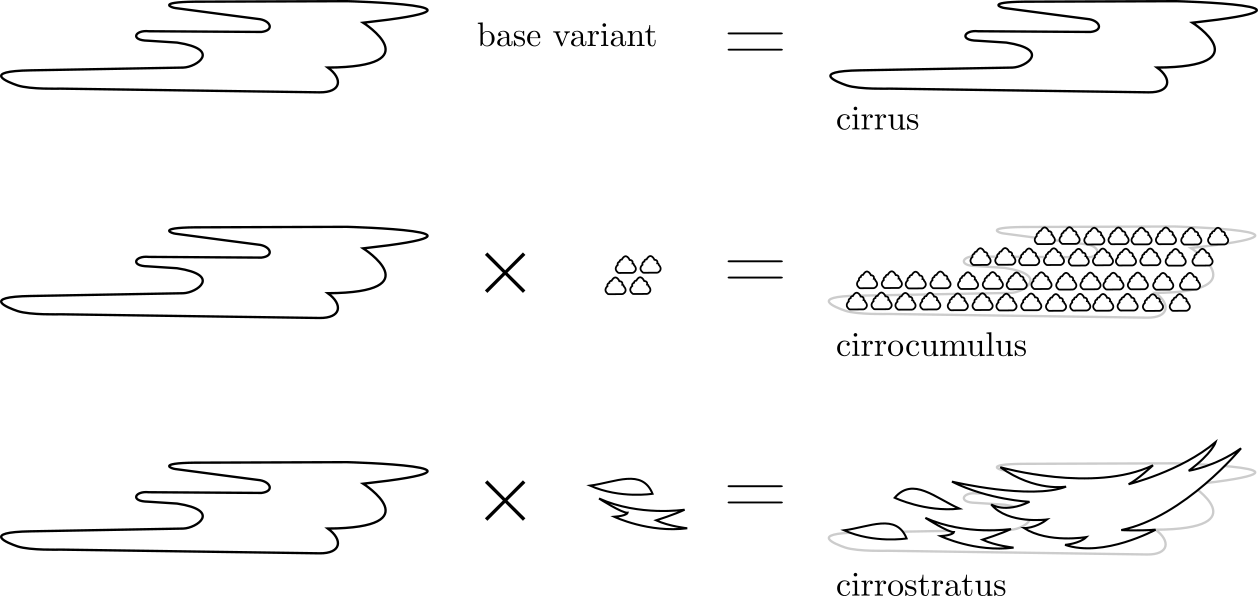
\includegraphics[width=\linewidth]{cloudlayers/cirruslayer.png}
    \caption{A breakdown of the cirrus cloud layer.}
    \label{img:cloudlayer:cirrus}
\end{figure}

\subsubsection{Alto Layer}
The middle layer consists of altostratus and altocumulus clouds, the latter mainly being formed by dissipation of the former one.
Since they have many shared characteristics, apart from the puffiness, they are predestined to be combined.
\\
Given a \gls{shader} is flexible enough to render altostratus clouds, then it is also able to render altocumulus, with only few adjustements necessary.

\begin{figure}[H]
    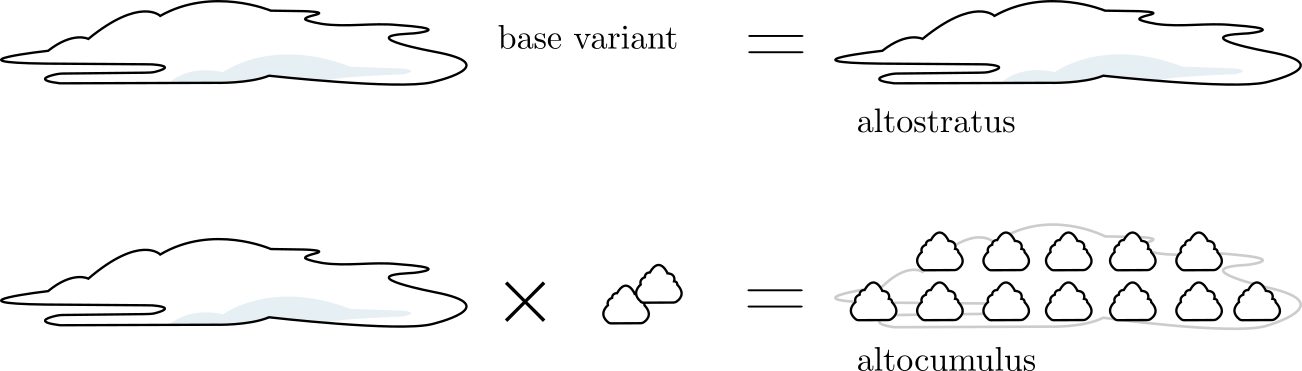
\includegraphics[width=\linewidth]{cloudlayers/altolayer.png}
    \caption{A breakdown of the alto cloud layer.}
    \label{img:cloudlayer:alto}
\end{figure}